\documentclass{article}

\usepackage[T1]{fontenc}    %Schriftart des Dokumentes
\usepackage[british]{babel} %Dokumentensprache, hier Deutsch
\usepackage{amsmath, amssymb, stmaryrd} %mathematische Schriftzeichen
\usepackage{graphicx} %Einfügen von Grafiken
\usepackage{wrapfig}
\usepackage{bm}

\setlength{\parindent}{0pt} %Einrückung von Absätzen auf null gesetzt
\setlength{\parskip}{10pt} %Abstand zischen Absätzen auf 10pt gesetzt

\title{Experiment 15: Inclined Plane}
\author{Matthias Kuntz}
\date{22.09.2023}

\begin{document}

\maketitle

%-------------------------EINLEITUNG-------------------------
\section{Introduction}

In this experiment we will observe different types of cylinders rolling down an inclined plane. We will measure the time it takes for the cylinders to travel certain distances down the incline to determine their acceleration, comparing the results to the theoretical values we will be calculating. Finally, we will record their speed after rolling down the incline to observe the conservation of energy.  

\subsection{Basics}

A real cylinder rolling down an incline experiences friction. We can determine that this friction force $F_R$  exerts a torque $\tau$ on the rolling cylinder, dependent on the radius $r$:

\begin{equation}
    \tau = F_R r = I \frac{d\omega}{dt}
    \label{eq:1}
\end{equation}

Here, $I$ is the moment of inertia and $\omega$ the angular velocity of the rolling body. We use the rolling condition $v_c =r \omega$, with $v_c$ being the velocity of the centre of gravity, to obtain

\begin{equation}
    \begin{split}
        \tau = F_R r &= \frac{I}{r} \frac{dv_c}{dt} = \frac{I}{r} a_c \\
        \iff F_R &= \frac{I}{r^2} a_c.
    \end{split}
    \label{eq:2}
\end{equation}

Generally, we can derive the differential equation of the centre of gravity of a rolling body on an incline and using our determined friction force we can find the acceleration:

\begin{equation}
    \begin{split}
        ma_c &= md \sin{(\phi)} - F_R \\
        \iff ma_c &= md \sin{(\phi)} - \frac{I}{r^2} a_c \\ \\
        \implies a_c &= \frac{mg \sin{(\phi)}}{m + \frac{I}{r^2}}
    \end{split}
    \label{eq:3}
\end{equation}

Using the definition of the moment of inertia 

\begin{equation}
    I = \int r^2 dm,
    \label{eq:4}
\end{equation}

we can determine the moments if inertia of a solid cylinder $I_s$ and a hollow cylinder $I_h$:

\begin{equation}
    \begin{split}
        I_s &= \frac{1}{2} MR^2 \\
        I_h &= \frac{1}{2} M(R_i^2 + R_o^2) \\
    \end{split}
    \label{eq:5}
\end{equation}

Here, the index $i$ means inner and $o$ outer radius. 

When analysing the energy conservation, we need to determine the energy of the single cylinders. For this, we can determine the entire energy $E$ by adding up translational, rotational, and potential energy:

\begin{equation}
    E = \frac{1}{2} mv^2 + \frac{1}{2} I \omega^2 + mgh
    \label{eq:6}
\end{equation}

Where $v$ is the translational velocity and h the height the body rolls down. If energy is conserved, the body should have a kinetic energy equal to the starting potential energy after rolling down the incline which means 

\begin{equation}
    \frac{1}{2} mv^2 + \frac{1}{2} I \omega^2 = mgh.
    \label{eq:7}
\end{equation}

\subsection{Experiment Setup}

A sketch of the experiment setup is given on the next page in the measurement protocol.

We will start by measuring all relevant information like radii and masses. Then we set up the light barriers on the incline and measure their distances from the starting position where the cylinders start rolling. The light barriers are connected to a terminal which shows the times it takes for an object to pass through the barrier from the moment the bar at the starting position is released. We will record these times for both the solid and hollow cylinders five times each. Finally, we will place two light barriers at the beginning and end of the level plane after the incline, measure their distance apart from another and record their measured times for both cylinders five times.

%---------------VERSUCHSPROTOKOLL MIT MESSDATEN---------------
\newpage

\section{Measurement Protocol}

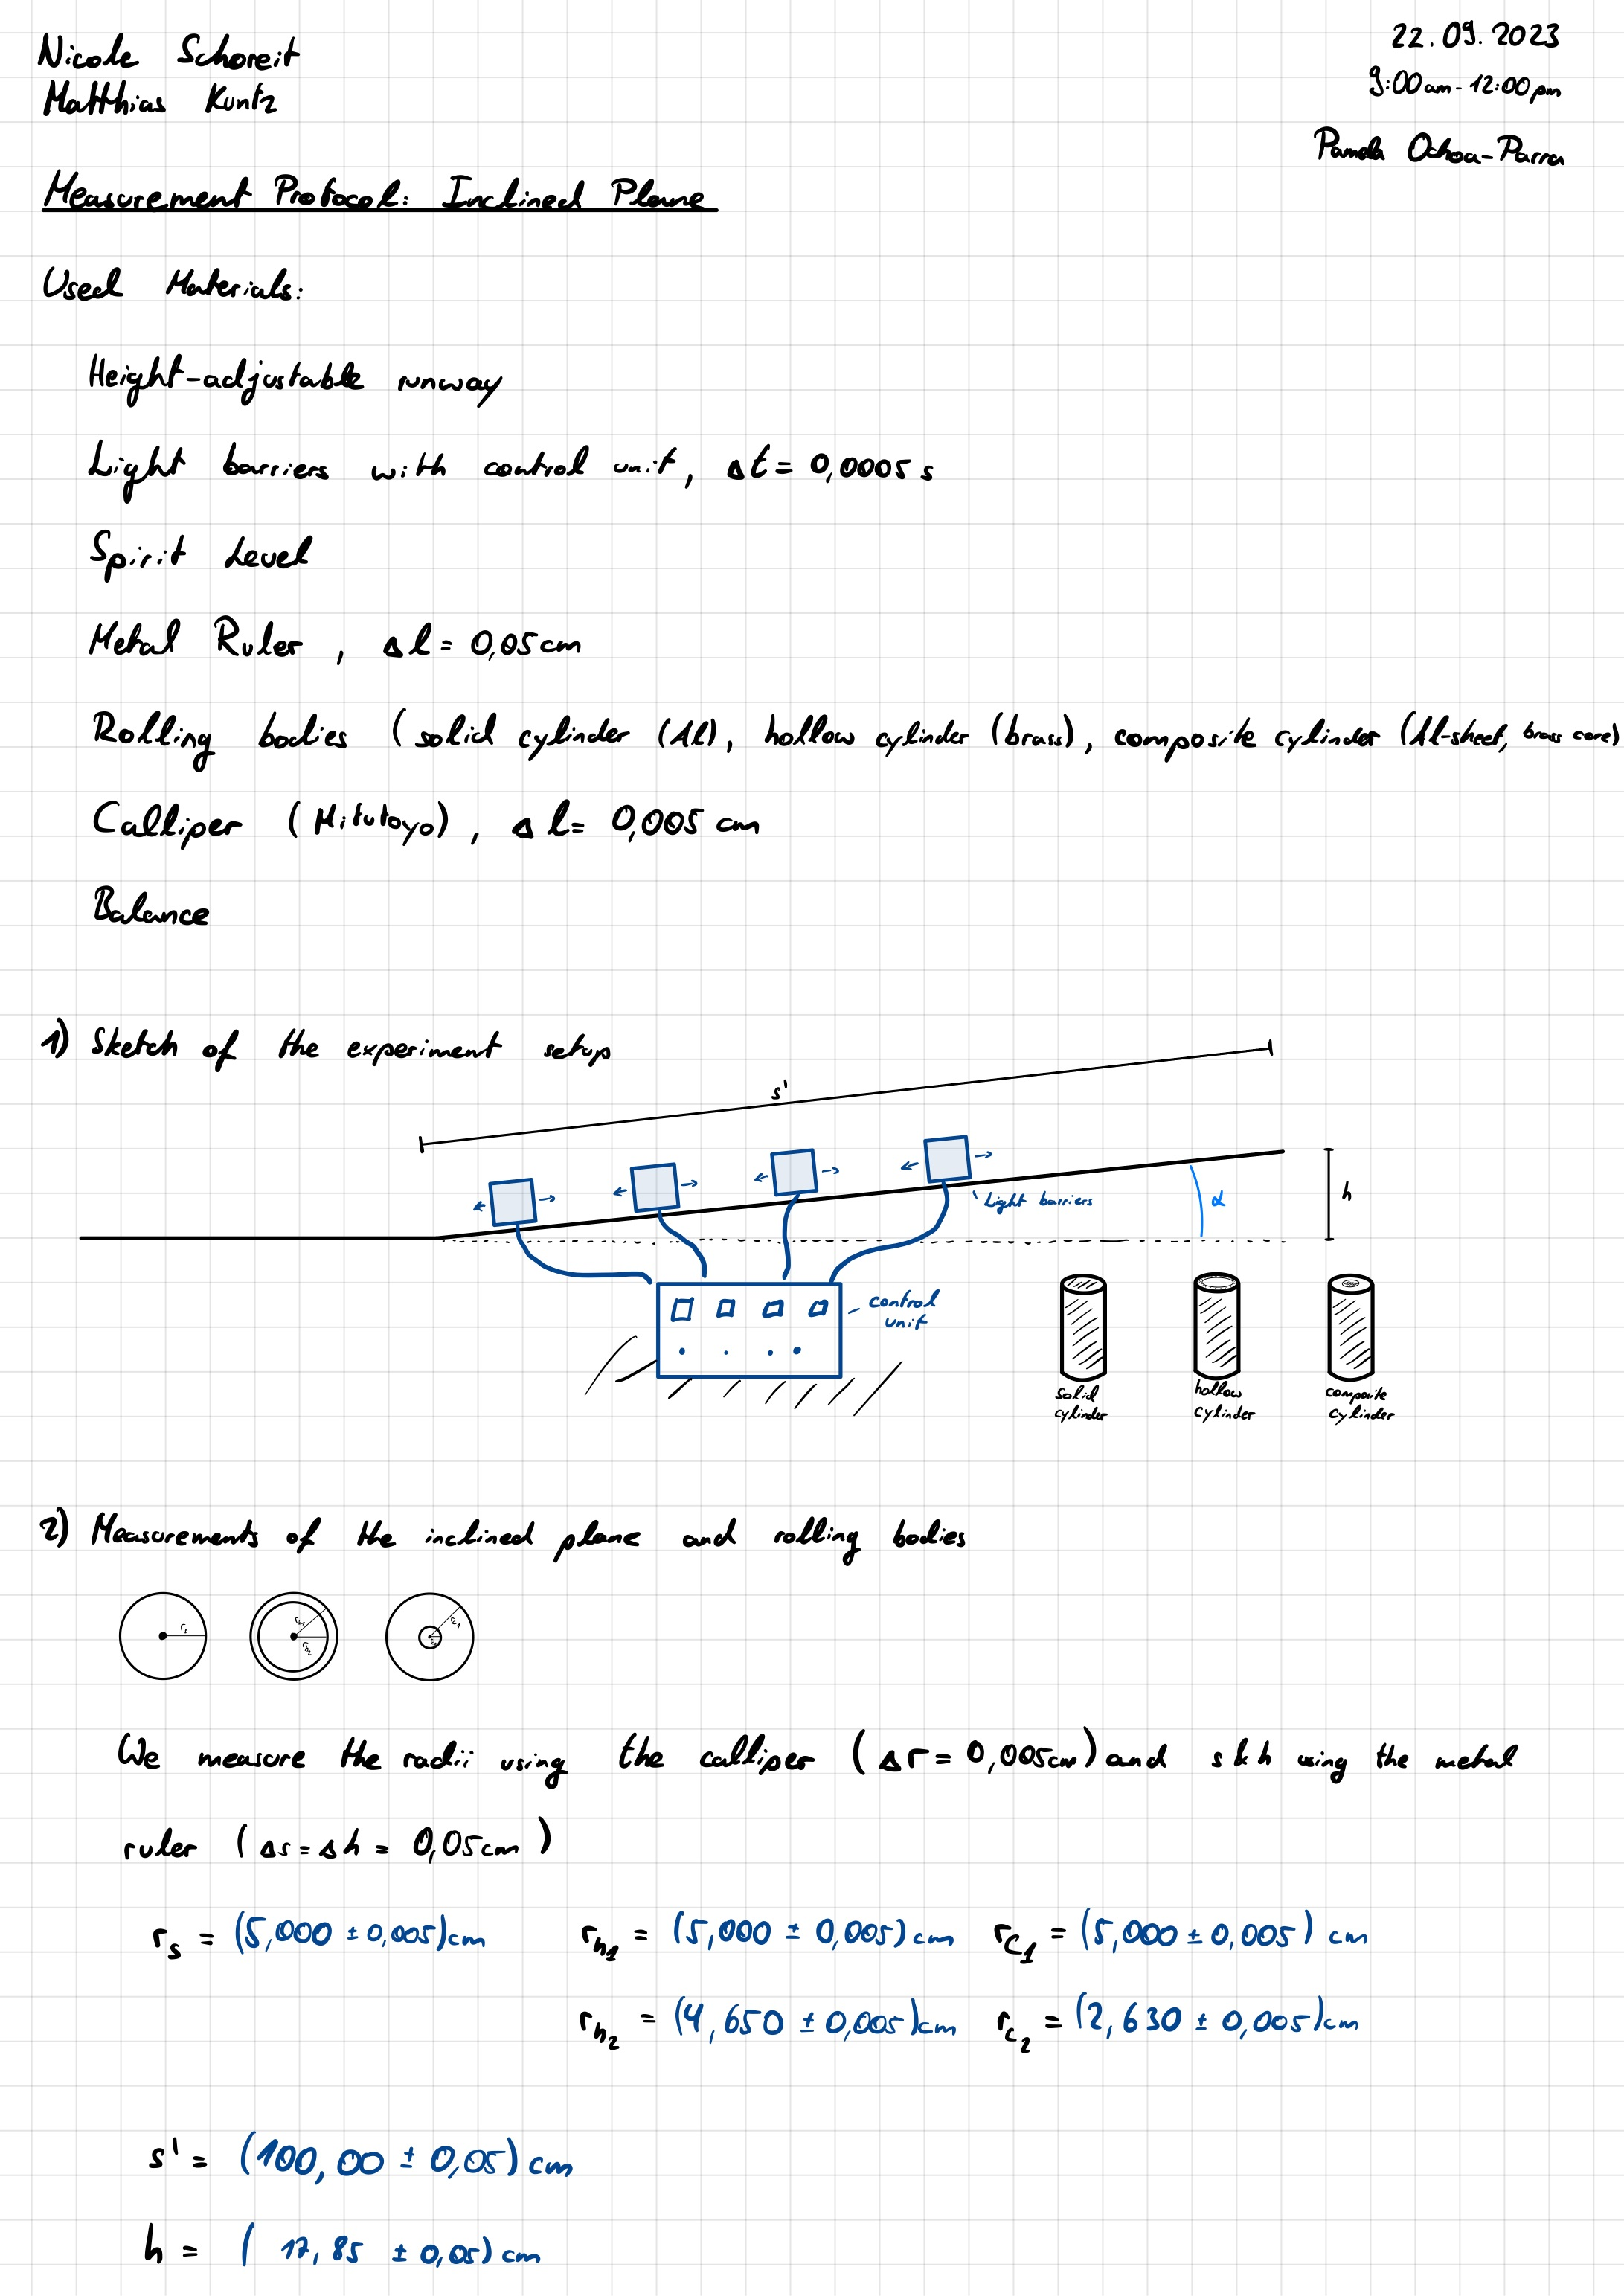
\includegraphics[width=\textwidth]{graphics/mess1.jpg}
\newpage
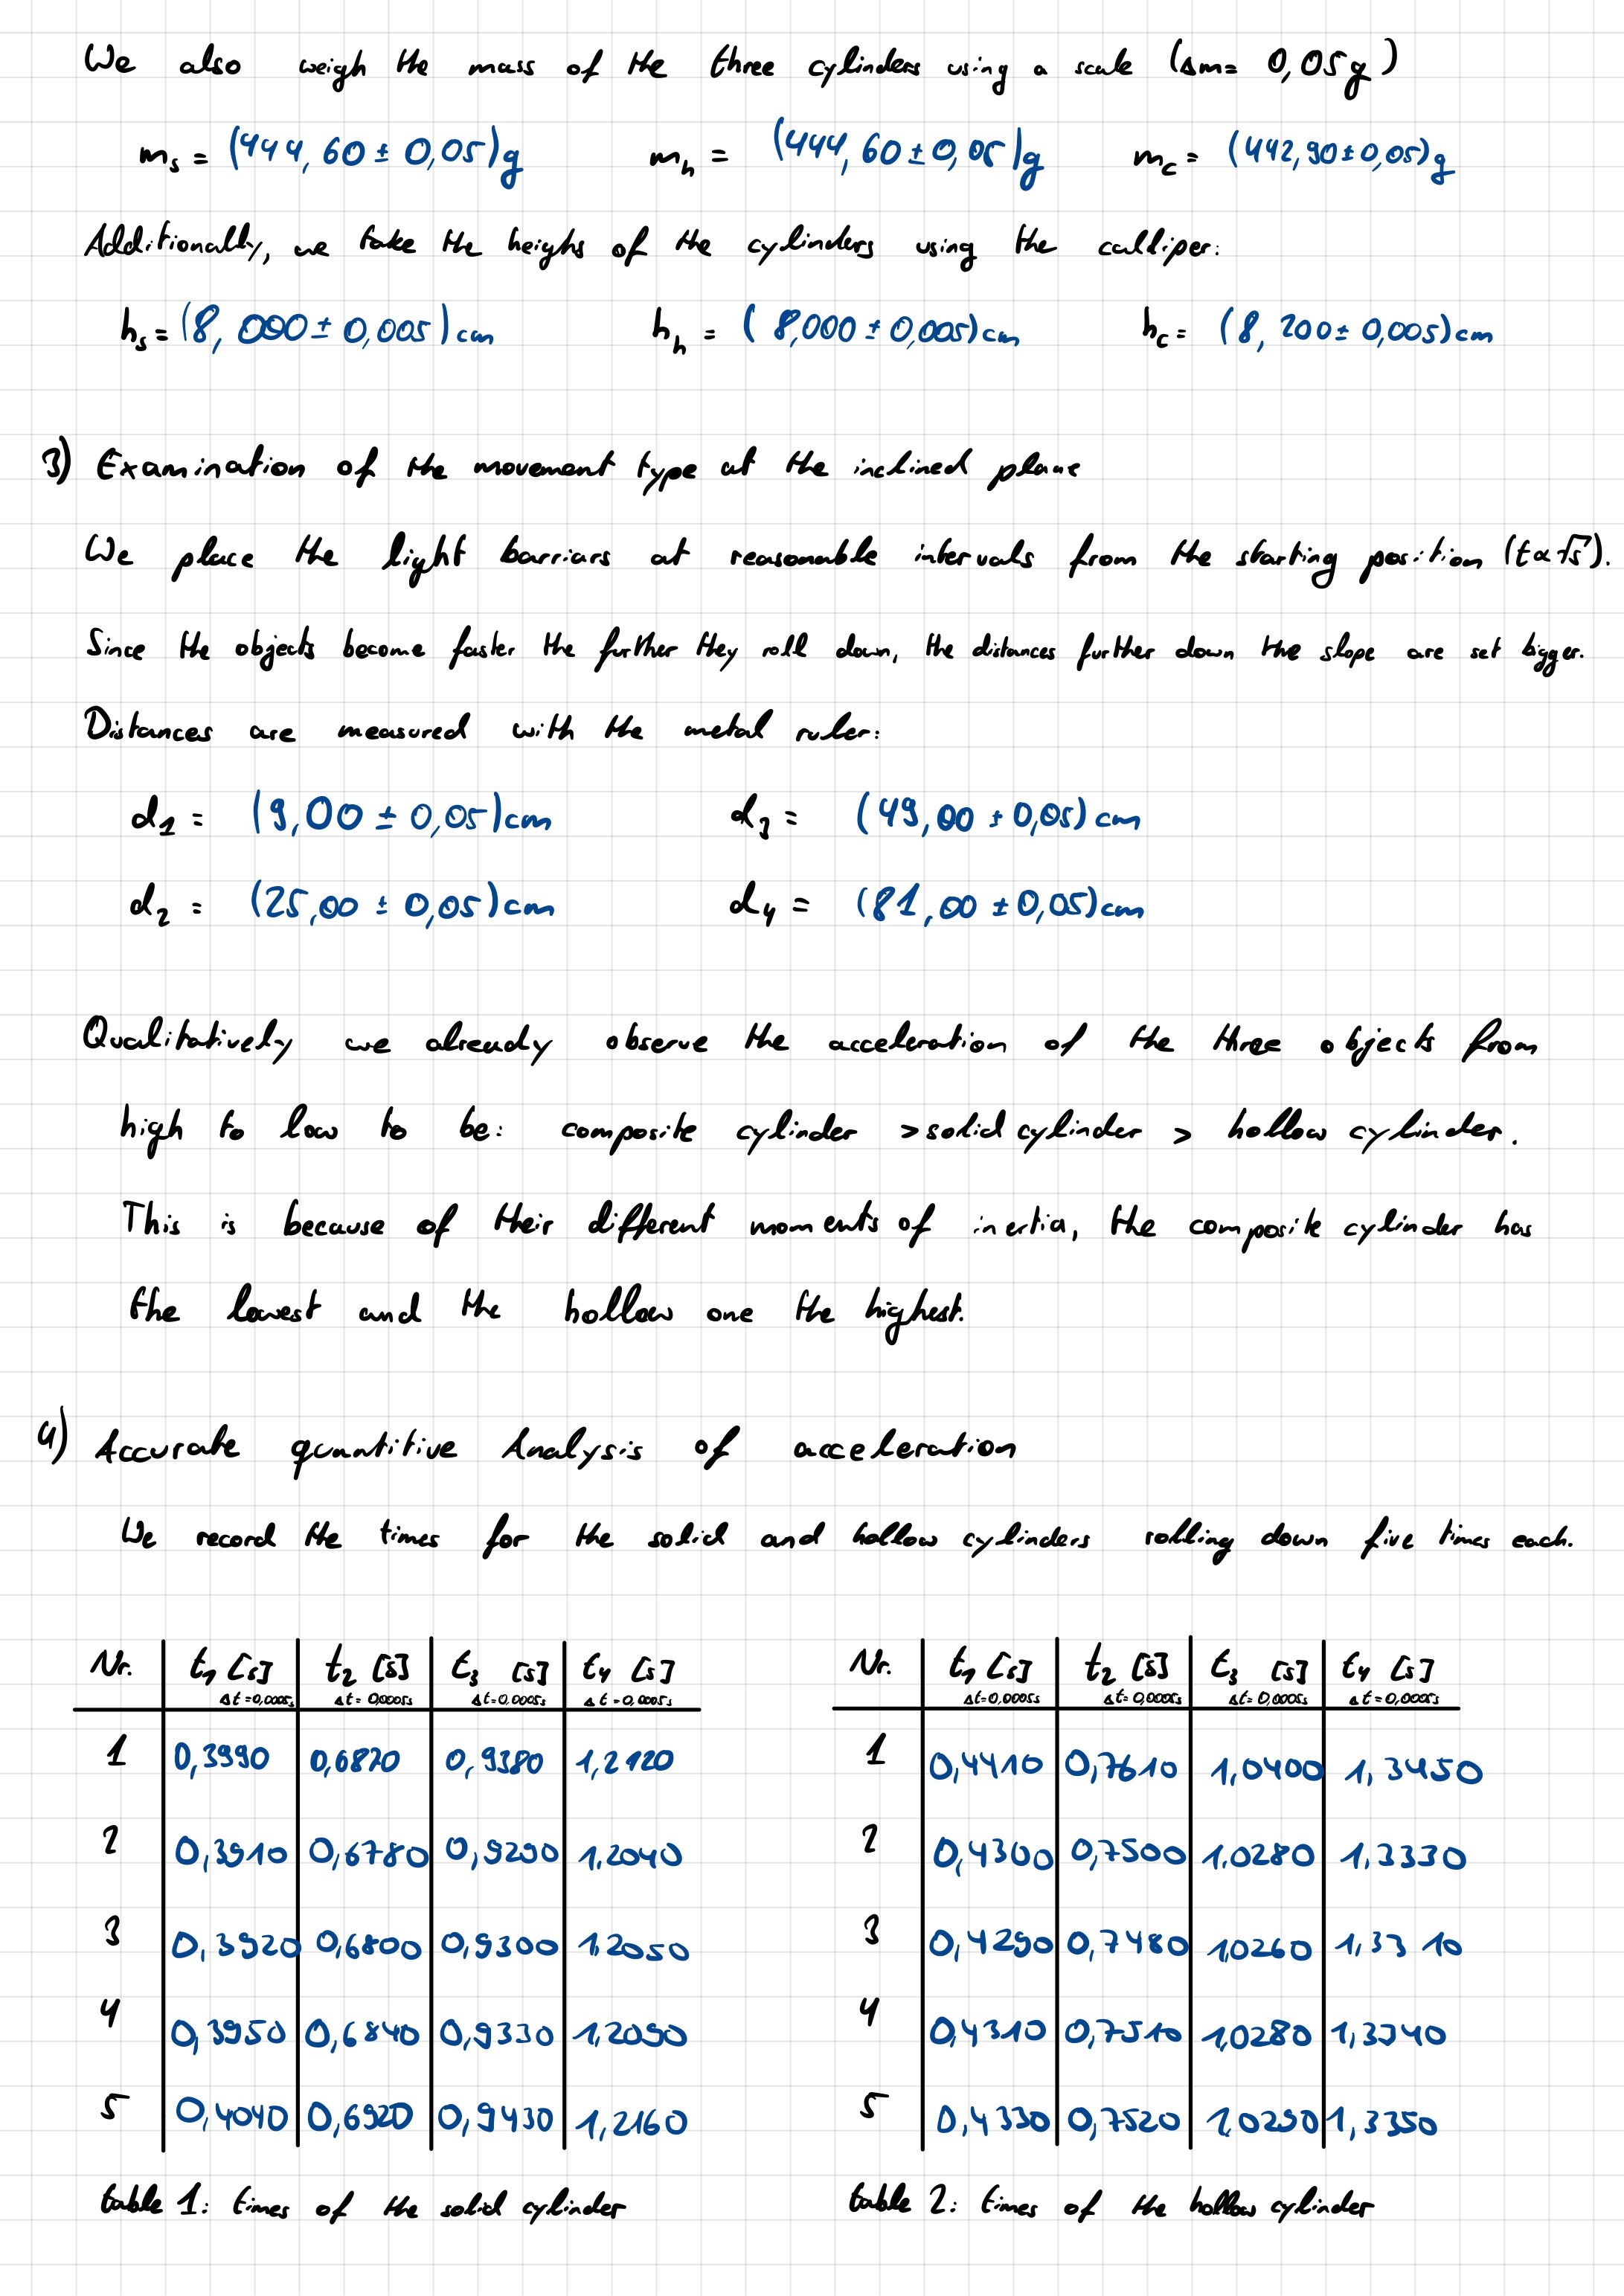
\includegraphics[width=\textwidth]{graphics/mess2.jpg}
\newpage
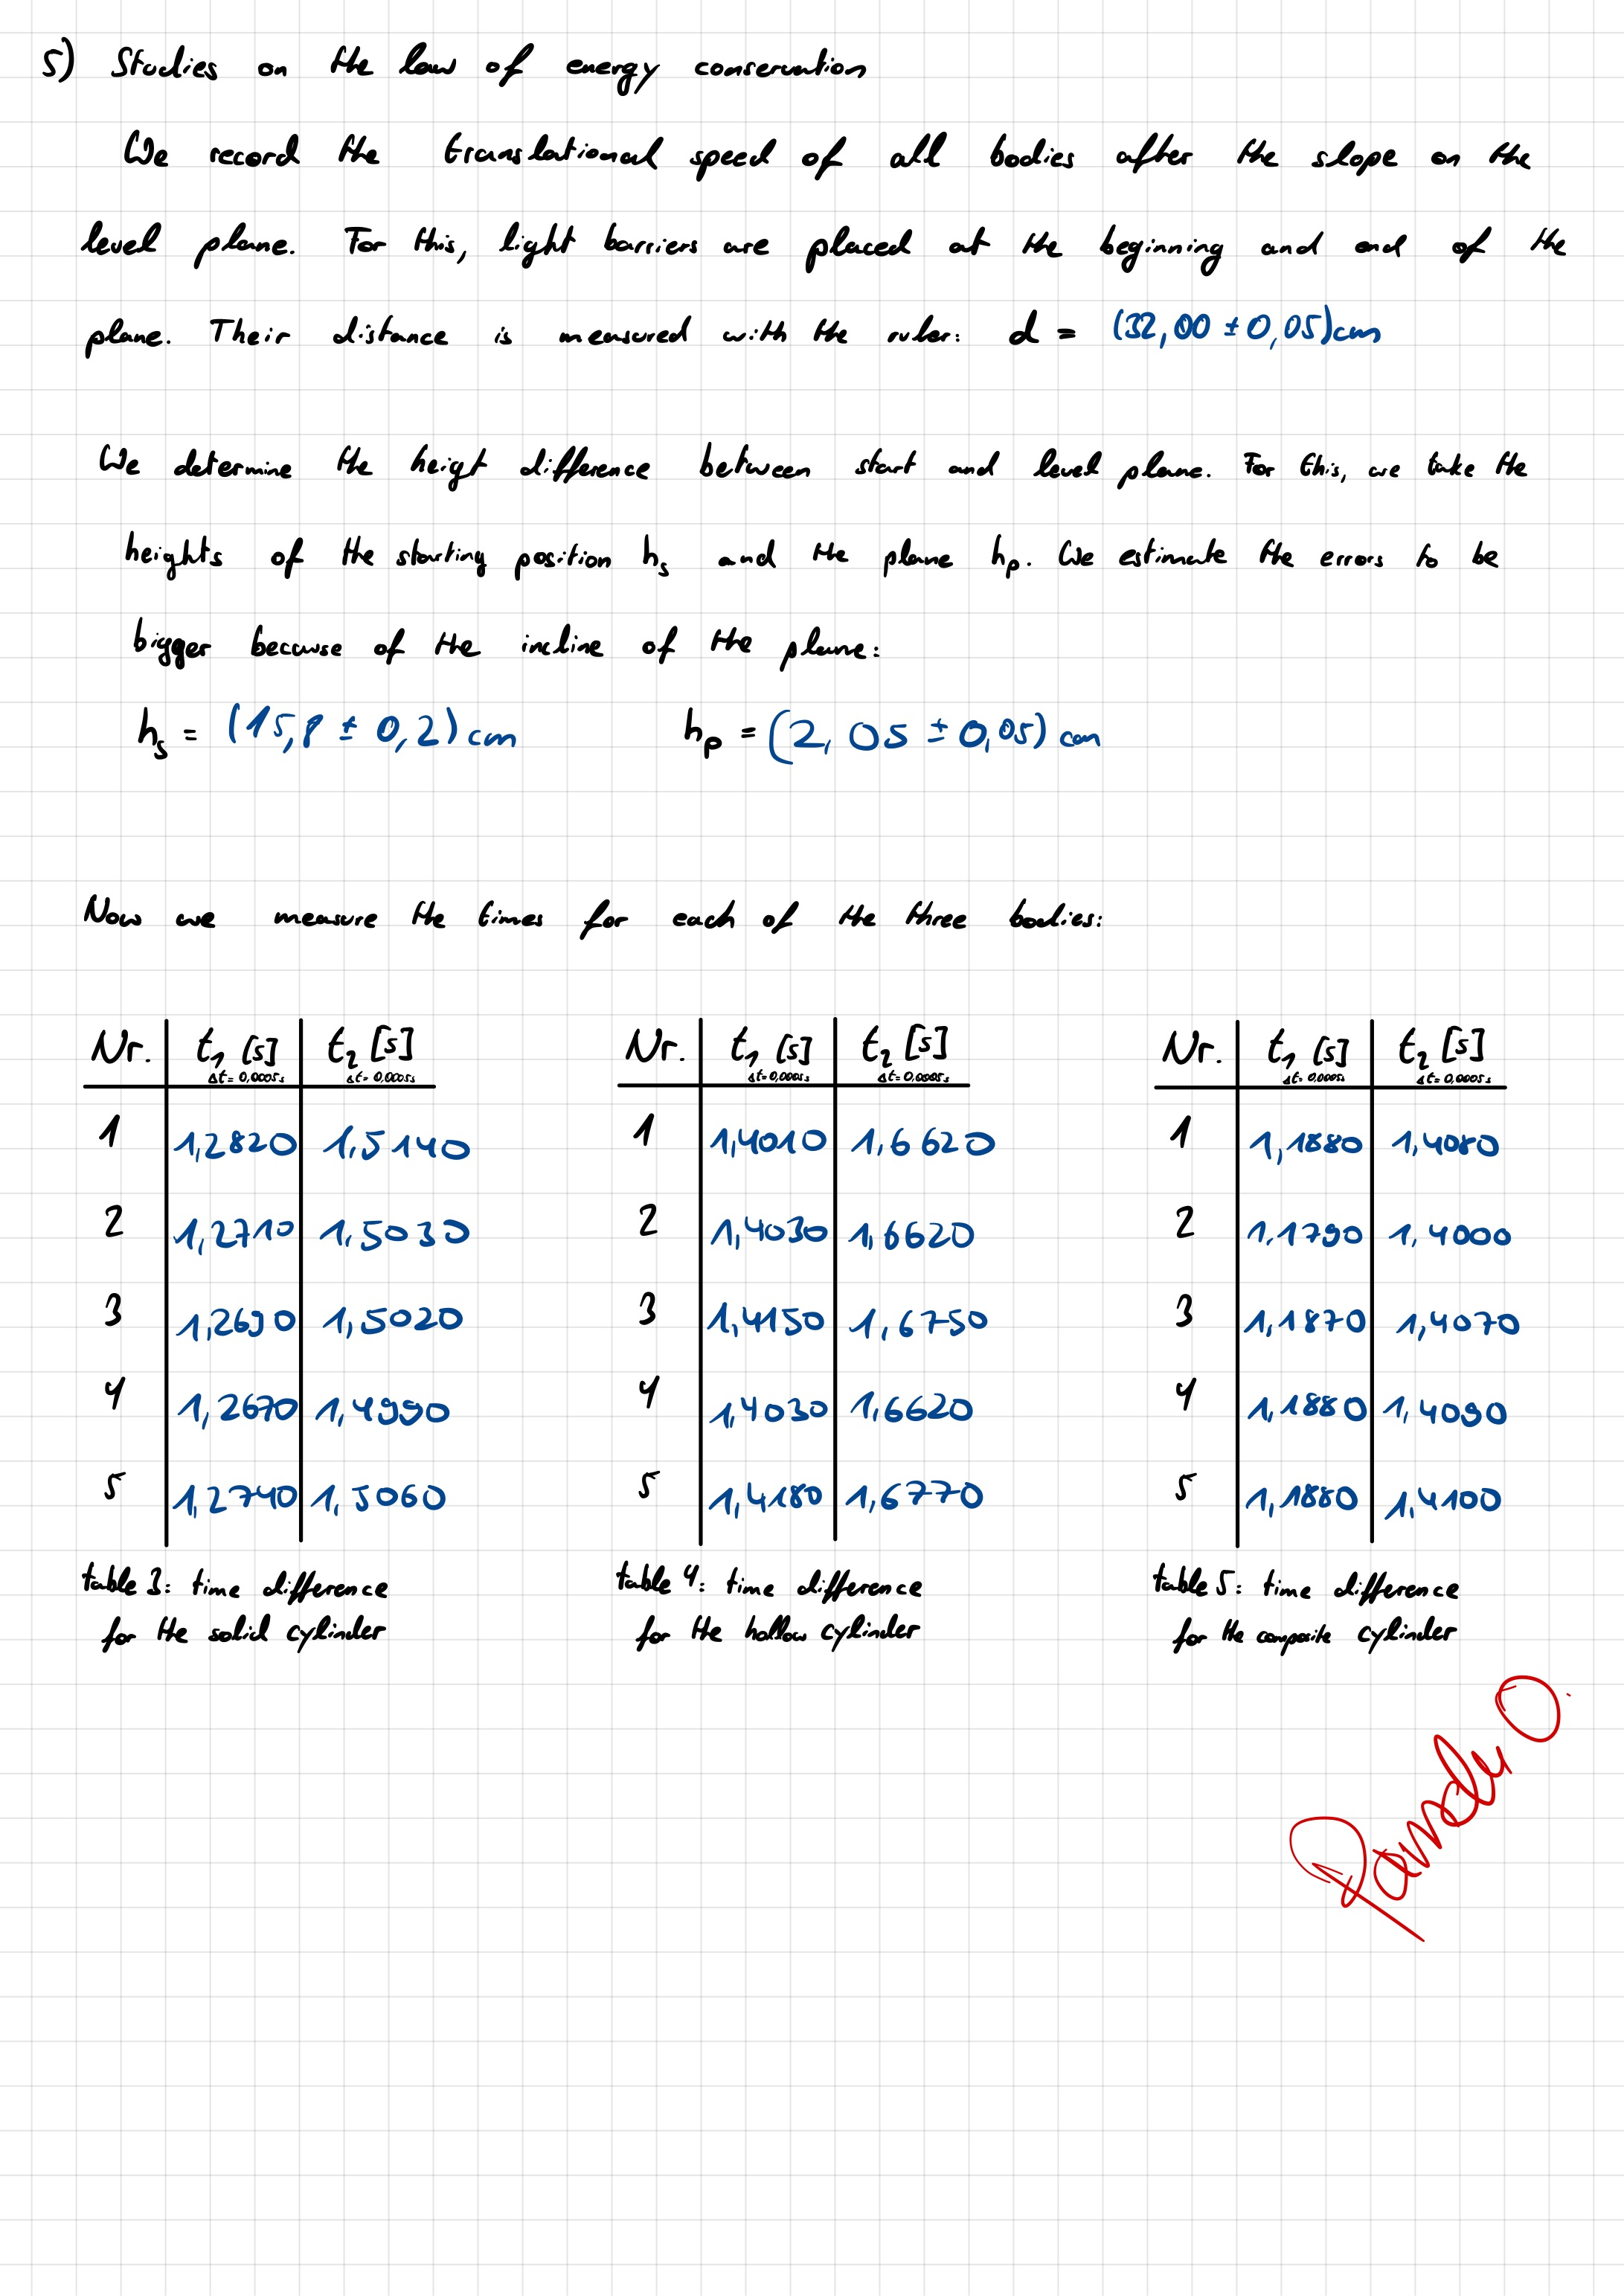
\includegraphics[width=\textwidth]{graphics/mess3.jpg}
\newpage

\addtocounter{table}{5}

%-------------------------AUSWERTUNG-------------------------
\section{Evaluation}

In this evaluation all errors, unless otherwise specified, are calculated using Gaussian error propagation. Meaning, if a value $F$ is calculated by formula $f(a_1, ..., a_n)$, the error $\Delta F$ is given as

\begin{equation}
    \Delta F = \sqrt{\sum_n \left( \frac{\partial f}{\partial a_n} \cdot \Delta a_n \right)^2}.
\end{equation}

We start by determining the angle of the incline $\alpha$ from the measurements taken in part 2:

\begin{equation}
    \begin{split}
        \sin{\alpha} &= \frac{h}{s'} \iff \alpha = \arcsin{\frac{h}{s'}} \\
        \Delta \alpha &= \sqrt{\left( \frac{1}{s' \sqrt{1-\frac{h^2}{s'^2}}} \cdot \Delta h \right)^2 + \left( \frac{h}{s'^2 \sqrt{1-\frac{h^2}{s'^2}}} \cdot \Delta s' \right)^2} \\ \\
        \implies \alpha &= (10,2824 \pm 0,0005)^\circ
    \end{split}
    \label{eq:99}
\end{equation}

\subsection{Determining the accelerations}

In order to calculate the acceleration, we use $s=\frac{a}{2}t^2$ to identify the acceleration $a$ as the slope of a line $s(t^2)$ times two. When we want to plot this graph, we take the measurements from tables 1 and 2. For the plot, we calculate the mean values $\overline{t}$ and their errors $\Delta \overline{t}$ using

\begin{equation}
    \Delta \overline{t} = \sqrt{(\Delta t)^2 + (\Delta t_\sigma)^2},
    \label{eq:98}
\end{equation}

where $\Delta t$ is the measurement error given in the protocol and $\Delta t_\sigma$ is the standard error of the mean. These values will then be squared and their errors calculated accordingly:

\begin{equation}
    \Delta \overline{t}^2 = 2 \overline{t} \cdot \Delta \overline{t}
\end{equation}

In doing all that, we get the values shown in table \ref{tab:1}, which are plotted in the diagrams shown in figures \ref{fig:solid} and \ref{fig:hollow}. 

\begin{table} [!ht]
    \centering
    \begin{tabular}{c|c|c|c|c}
        \hline
        \textbf{cylinder} & \textbf{Nr.} & $\bm{\overline{t}}$ [s] & $\bm{\overline{t}^2}$ [s] & $d$ [cm]\\ \hline
        solid & 1 & $0,3962 \pm 0,0024$ & $0,1570 \pm 0,0019$ & $9,00 \pm 0,05$ \\
         & 2 & $0,686 \pm 0,004$ & $0,471 \pm 0,005$ & $25,00 \pm 0,05$ \\
         & 3 & $0,9346 \pm 0,0027$ & $0,873 \pm 0,005$ & $49,00 \pm 0,05$ \\
         & 4 & $1,2092 \pm 0,0023$ & $1,462 \pm 0,006$ & $81,00 \pm 0,05$ \\ \hline
        hollow & 1 & $0,4328 \pm 0,0022$ & $0,1873 \pm 0,0019$ & $9,00 \pm 0,05$ \\
         & 2 & $0,7524 \pm 0,0023$ & $0,566 \pm 0,003$ & $25,00 \pm 0,05$ \\
         & 3 & $1,043 \pm 0,015$ & $1,09 \pm 0,03$ & $49,00 \pm 0,05$ \\
         & 4 & $1,3356 \pm 0,0025$ & $1,784 \pm 0,007$ & $81,00 \pm 0,05$ \\ \hline
    \end{tabular}
    \caption{values for the plot of acceleration}
    \label{tab:1}
\end{table}

\newpage

We take the values from the diagram to determine the accelerations and their errors according to

\begin{equation}
    \begin{split}
        a &= 2 \cdot \frac{\Delta d}{\Delta t^2} \\
        \Delta a &= 2 \cdot \left| \frac{\Delta d}{\Delta t^2} - \frac{\Delta d_f}{\Delta t_f^2} \right|
    \end{split}
    \label{eq:97}
\end{equation}

We calculate the following results, where the index $s$ indicates the solid and $h$ the hollow cylinder:

\begin{equation}
    \begin{split}
        \bm{a_s} &= \bm{(1,106 \pm 0,005) \frac{\textbf{m}}{\textbf{s}^2}} \\
        \bm{a_h} &= \bm{(0,900 \pm 0,005) \frac{\textbf{m}}{\textbf{s}^2}} \\
    \end{split}
    \label{res:a}
\end{equation}

\newpage

To compare these values we calculate the accelerations $a'$ using equation \ref{eq:3} and the according moments of inertia in equation \ref{eq:5} as well as the values for the masses and radii recorded in part 1 of the measurement protocol. We use 

\begin{equation}
    \begin{split}
        \Delta I_s &= \sqrt{\left( \frac{1}{2}R^2 \cdot \Delta M \right)^2 + (MR \cdot \Delta R)^2} \\
        \Delta I_h &= \sqrt{\left( \frac{1}{2}(R_i^2 + R_o^2) \cdot \Delta M \right)^2 + (MR_i \cdot \Delta R_i)^2 + (MR_o \cdot \Delta R_o)^2} \\ \\
        \Delta a' &= \frac{gmr^2}{(I+mr^2)^2} \Biggl[ \left( (I+mr^2)\cos{(\alpha)} \cdot \Delta \alpha \right)^2 + \left( \frac{I \sin{(\alpha)}}{m} \cdot \Delta m \right)^2 \\
        &+ \left( \sin{(\alpha)} \cdot \Delta I \right)^2 + \left( \frac{2I \sin{(\alpha)}}{r} \cdot \Delta r \right)^2 \Biggr]^{\frac{1}{2}}        
    \end{split}
    \label{eq:err1}
\end{equation} 

for the according errors. Doing so will yield

\begin{equation}
    \begin{split}
        \bm{I_s} &= \bm{(0,56 \pm 0,06) \cdot 10^{-3} \textbf{kg} \cdot \textbf{m}}^2 \\
        \bm{I_h} &= \bm{(1,04 \pm 0,12) \cdot 10^{-3} \textbf{kg} \cdot \textbf{m}}^2 \\
    \end{split}
\end{equation}

and

\begin{equation}
    \begin{split}
        \bm{a'_s} &= \bm{(1,167 \pm 0,003) \frac{\textbf{m}}{\textbf{s}^2}} \\
        \bm{a'_h} &= \bm{(0,9061 \pm 0,0026) \frac{\textbf{m}}{\textbf{s}^2}} \\
    \end{split}
    \label{res:a'}
\end{equation}

We can compare the values $a$ and $a'$ using the standard deviation:

\begin{equation}
    \begin{split}
        \sigma &= \frac{|a-a'|}{\sqrt{(\Delta a)^2 + (\Delta a')^2}} \\
        \sigma_s &= 10,46 \\
        \sigma_h &= 1,08
    \end{split}
    \label{sigma:a-a'}
\end{equation}

The first value shows a significant deviation, the second is insignificant.

\begin{figure} [p]
    \centering
    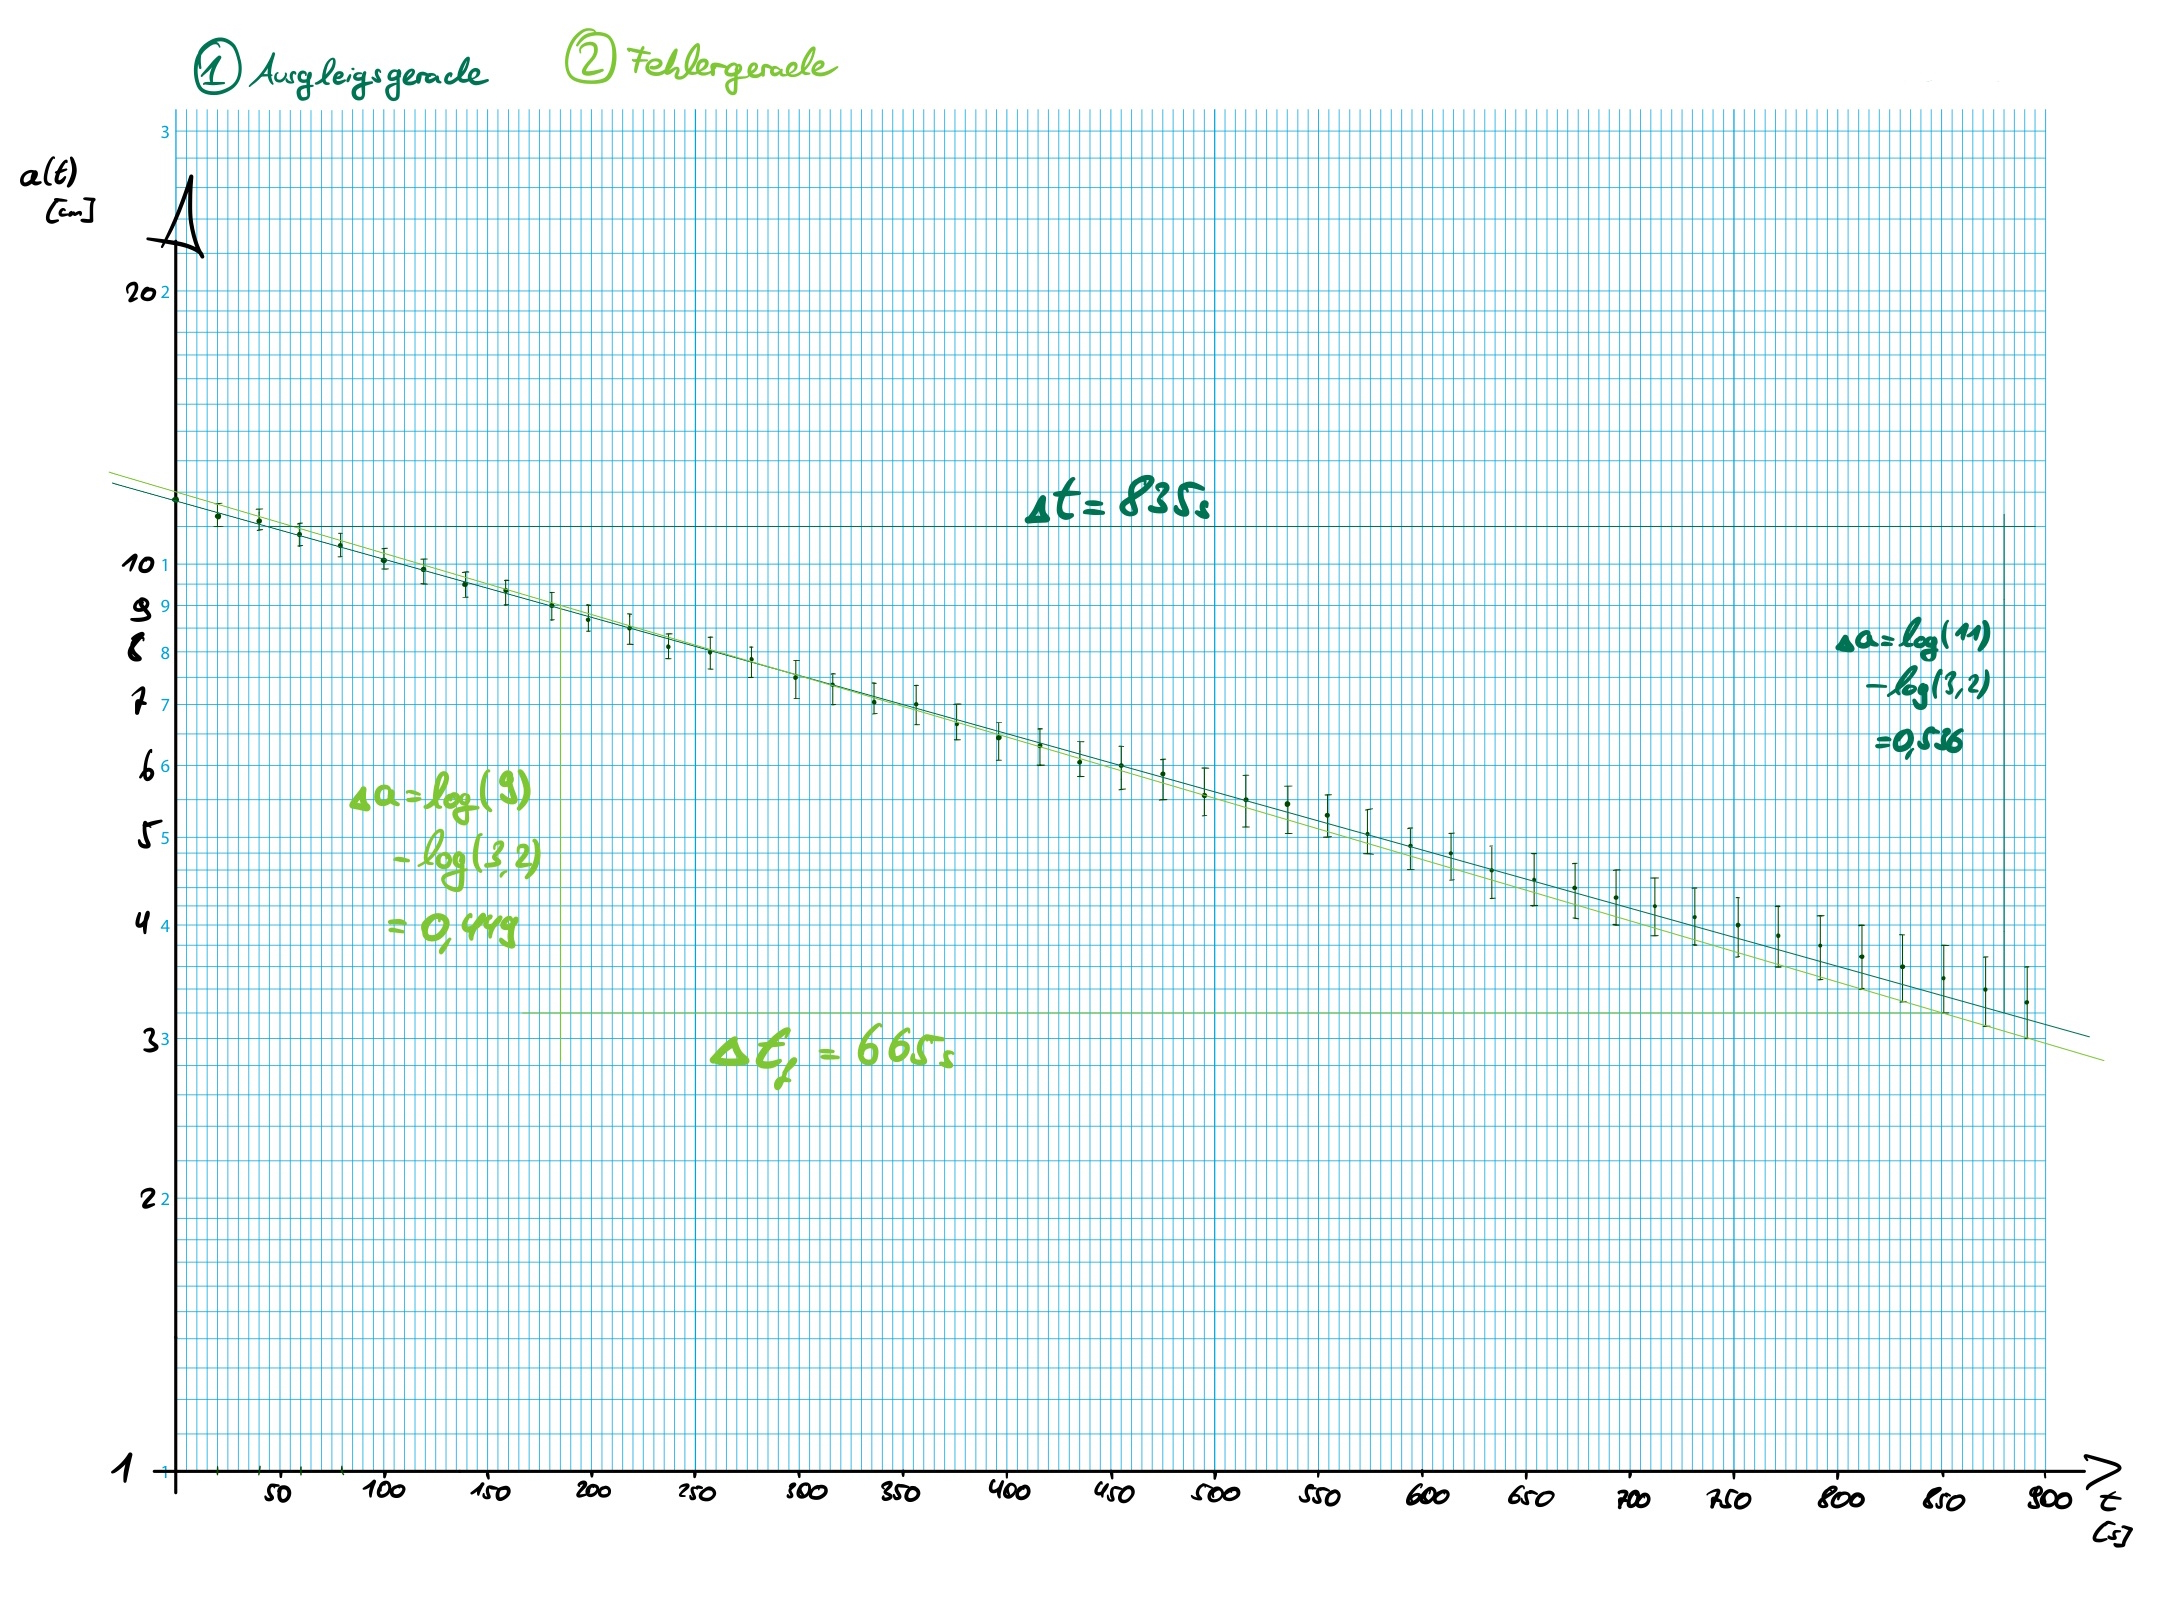
\includegraphics[width=\textwidth]{graphics/dia1.jpg}
    \caption{$s(t^2)$ for the solid cylinder}
    \label{fig:solid}
\end{figure}

\begin{figure} [p]
    \centering
    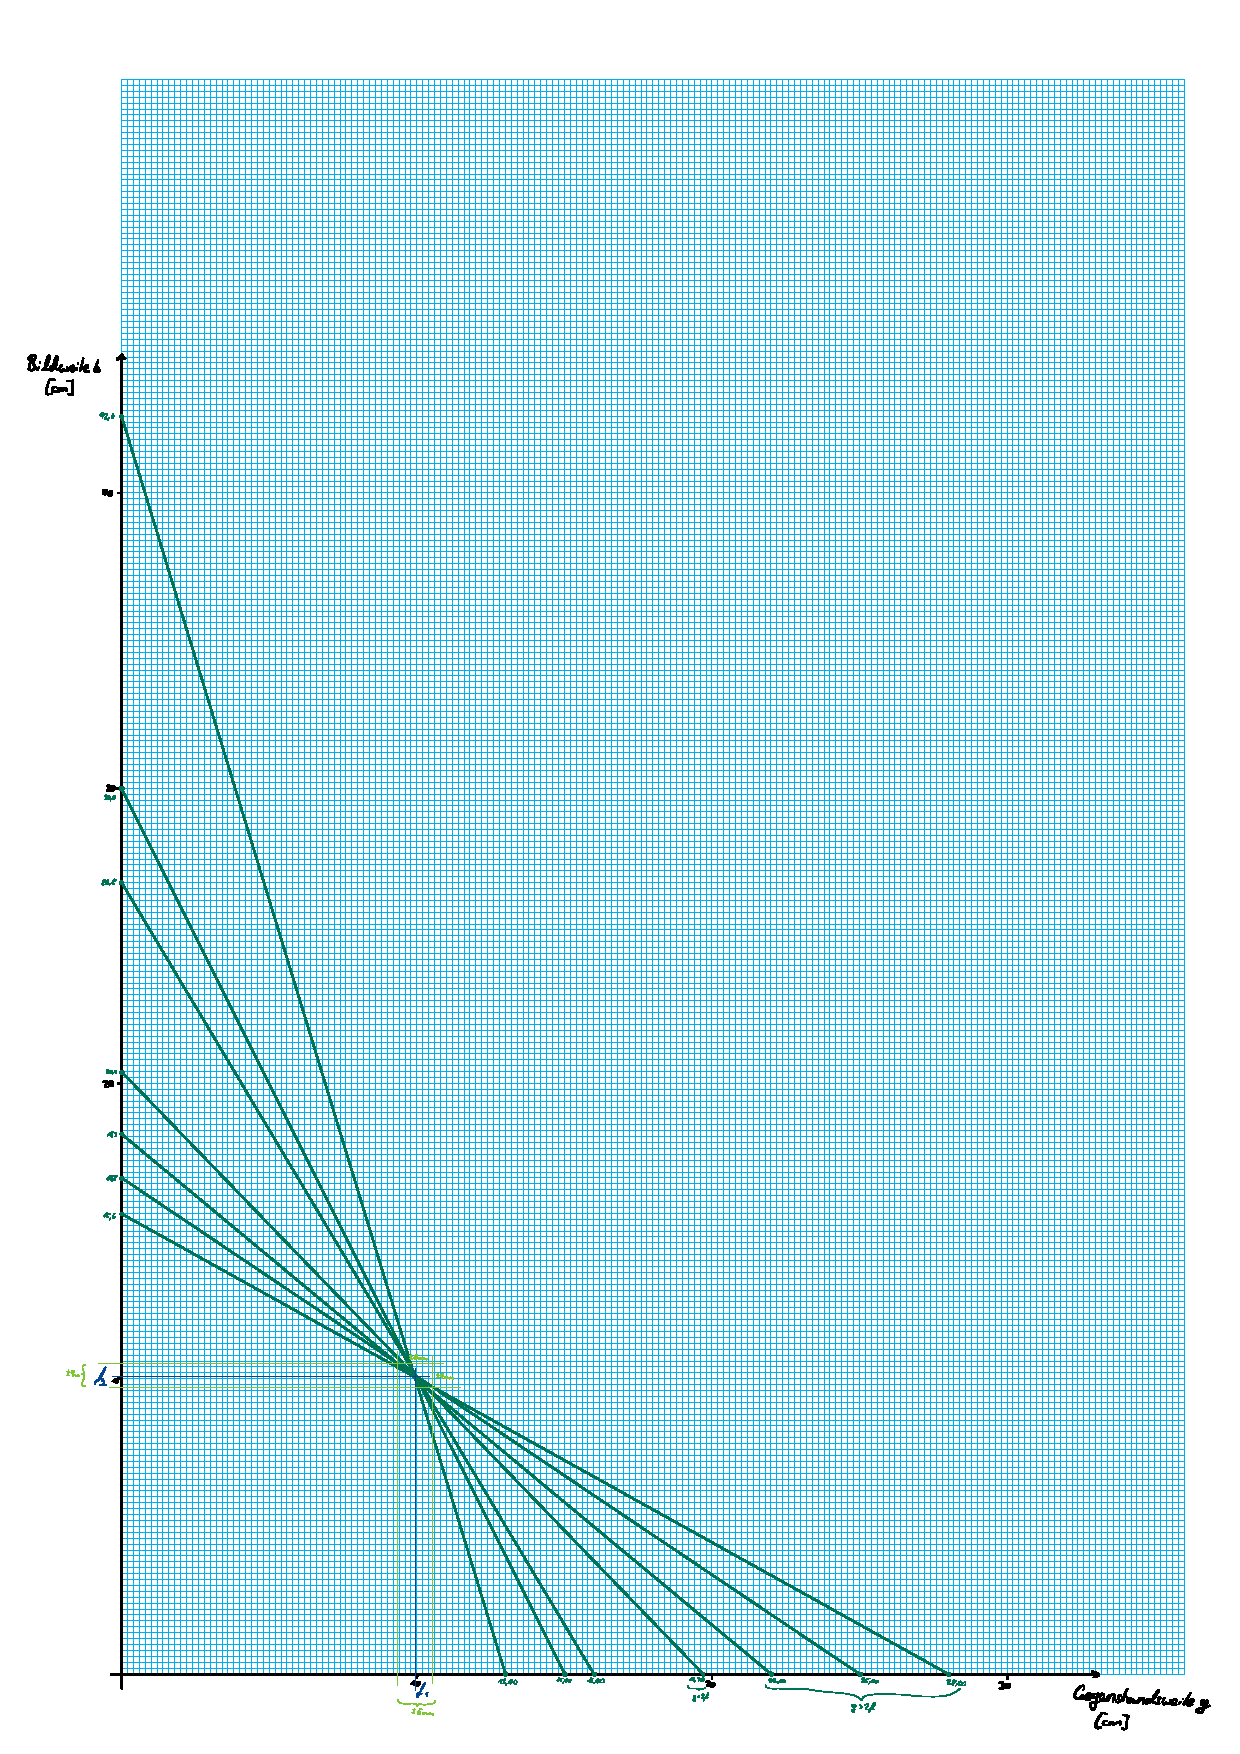
\includegraphics[width=\textwidth]{graphics/dia2.jpg}
    \caption{$s(t^2)$ for the hollow cylinder}
    \label{fig:hollow}
\end{figure}

\newpage

\subsection{Analysing energy conservation}

We start by calculating the kinetic energies of the solid and hollow cylinders defined in equation \ref{eq:7}. For this, we analyse the data recorded in tables 3 and 4. First, we calculate the difference between the values $t_1$ and $t_2$ as well as the error using

\begin{equation}
    \Delta (t_1 - t_2) = \sqrt{(\Delta t_1)^2 + (\Delta t_2)^2}.
\end{equation}

The same way as before, we determine the mean of the differences and its according error, analogous to equation \ref{eq:err1}. The results are presented in table \ref{tab:2}. 

\begin{table} [!ht]
    \centering
    \begin{tabular}{c|c|c|c}
        \hline
        \textbf{cylinder} & \textbf{Nr.} & $\bm{t_1-t_2}$ [s] & $\bm{\overline{t_1-t_2}}$ [s] \\ \hline
         & 1 & $0,2320 \pm 0,0007$ &  \\
         & 2 & $0,2330 \pm 0,0007$ &  \\
        solid & 3 & $0,2330 \pm 0,0007$ & $0,2324 \pm 0,0007$ \\
         & 4 & $0,2320 \pm 0,0007$ &  \\
         & 5 & $0,2320 \pm 0,0007$ &  \\ \hline
         & 1 & $0,2610 \pm 0,0007$ &  \\
         & 2 & $0,2590 \pm 0,0007$ &  \\
        hollow & 3 & $0,2600 \pm 0,0007$ & $0,2596 \pm 0,0008$ \\
         & 4 & $0,2590 \pm 0,0007$ &  \\
         & 5 & $0,2590 \pm 0,0007$ &  \\ \hline
    \end{tabular}
    \caption{times for the kinetic energy}
    \label{tab:2}
\end{table}

Now, using $d=vt$ we can determine the average translational velocity $v$ for each of the cylinders after rolling down the incline. For time we use the calculated mean value from table \ref{tab:2} and the distance will be the measured $d=(32,00\pm0,05)$cm:

\begin{equation}
    \begin{split}
        v=\frac{d}{t}, \ & \ \Delta v = v \sqrt{\left( \frac{\Delta d}{d} \right)^2 + \left( \frac{\Delta t}{t} \right)^2} \\ \\
        v_s &= (1,377 \pm 0,005) \frac{\text{m}}{\text{s}} \\
        v_h &= (1,233 \pm 0,004) \frac{\text{m}}{\text{s}} \\
    \end{split}
    \label{res:v}
\end{equation}

From the translational velocity we can derive the angular velocity:

\begin{equation}
    \begin{split}
        \omega = \frac{v}{r}, \ & \ \Delta \omega = \omega \sqrt{\left( \frac{\Delta v}{v} \right)^2 + \left( \frac{\Delta r}{r} \right)^2} \\ \\
        \omega_s &= (27,54 \pm 0,10) \frac{\text{1}}{\text{s}} \\
        \omega_s &= (24,66 \pm 0,10) \frac{\text{1}}{\text{s}} \\
    \end{split}
    \label{res:angularvel}
\end{equation}

Now we can calculate the kinetic energies $K$ of both cylinders using the calculated and recorded values:

\begin{equation}
    \begin{split}
        K &= \frac{1}{2} mv^2 + \frac{1}{2} I \omega^2 \\
        \Delta K &= \frac{1}{2} \sqrt{(v^2 \cdot \Delta m)^2 + (2mv \cdot \Delta v)^2 + (\omega^2 \cdot \Delta I)^2 + (2I \omega \cdot \Delta \omega)^2} \\
    \end{split}
\end{equation}

\begin{equation}
    \begin{split}
        \bm{K_s} &= \bm{(0,634 \pm 0,023)} \textbf{J} \\
        \bm{K_h} &= \bm{(0,65 \pm 0,04)} \textbf{J} \\        
    \end{split}
    \label{res:K}
\end{equation}

Since the masses of the two cylinders were measured the same, their potential energy $U$ is also the same. We determine the height $h = (0,1788 \pm 0,0021)$m according to the sketch in figure \ref{fig:sketchh}.

\begin{equation}
    \begin{split}
        U = mgh, \ \ & \ \ \Delta U = g \sqrt{(m \cdot \Delta h)^2 + (h \cdot \Delta m)^2} \\ \\
        \bm{U} &= \bm{(0,780 \pm 0,009)} \textbf{J}
    \end{split}
    \label{res:U}
\end{equation}

\begin{figure} [!ht]
    \centering
    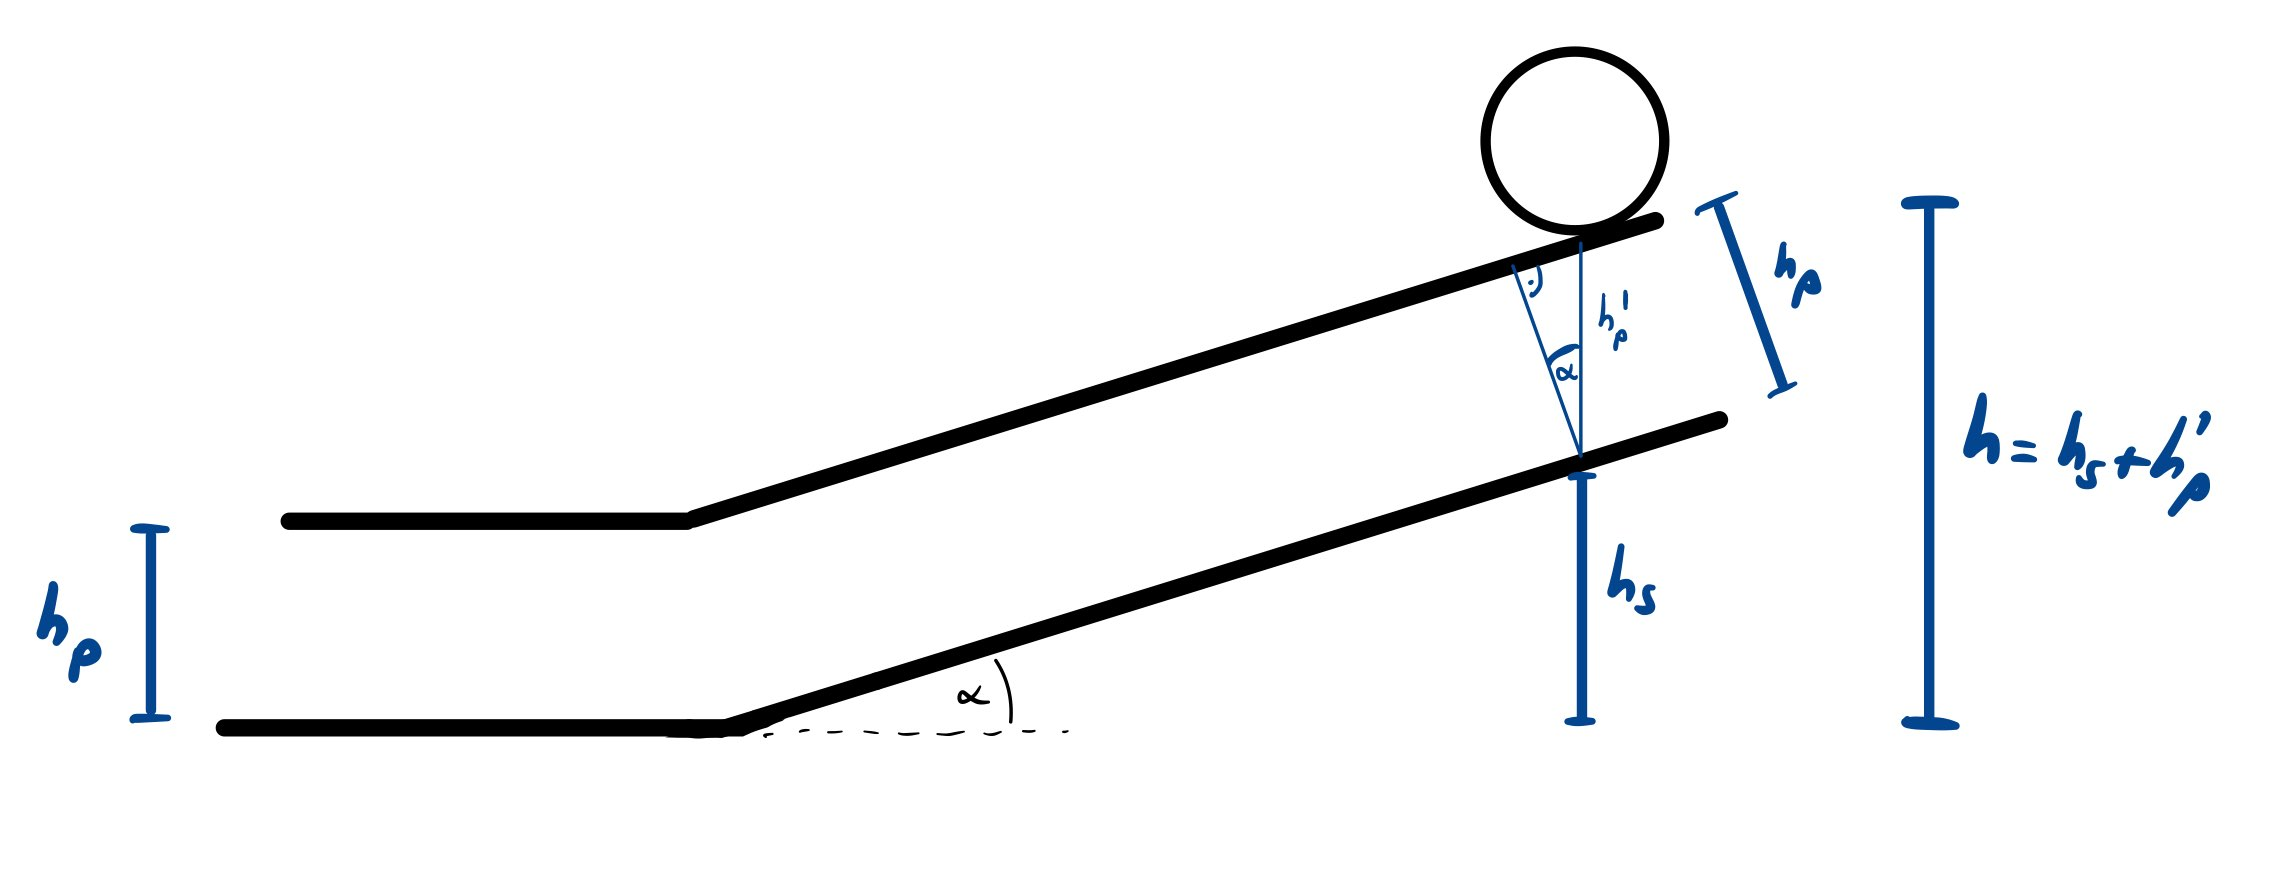
\includegraphics[width=7.5cm]{graphics/sketch15.jpg}
    \caption{sketch for determining the starting height $h$}
    \label{fig:sketchh}
\end{figure}

When comparing the values for $K$ and $U$ we get

\begin{equation}
    \begin{split}
        \sigma_s &= 5,91 \\
        \sigma_h &= 3,17 \\
    \end{split}
\end{equation}

which are both significant deviations.

\newpage
%---------------PRÄSENTATION DER ENDERGEBNISSE---------------
\section{Presentation of final results}

In this experiment we first determined the accelerations using our recorded times and additionaly using the given formula. The results were:

\begin{equation}
    \begin{split}
        \bm{a_s} &= \bm{(1,106 \pm 0,005) \frac{\textbf{m}}{\textbf{s}^2}} \\
        \bm{a_h} &= \bm{(0,900 \pm 0,005) \frac{\textbf{m}}{\textbf{s}^2}} \\        
    \end{split}
\end{equation}

\begin{equation}
    \begin{split}
        \bm{a'_s} &= \bm{(1,167 \pm 0,003) \frac{\textbf{m}}{\textbf{s}^2}} \\
        \bm{a'_h} &= \bm{(0,9061 \pm 0,0026) \frac{\textbf{m}}{\textbf{s}^2}} \\
    \end{split}
\end{equation}

Then, we calculated the kinetic and potential energies of the cylinders:

\begin{equation}
    \begin{split}
        \bm{K_s} &= \bm{(0,634 \pm 0,023)} \textbf{J} \\
        \bm{K_h} &= \bm{(0,65 \pm 0,04)} \textbf{J} \\        
    \end{split}
\end{equation}

\begin{equation}
    \begin{split}
        \bm{U} &= \bm{(0,780 \pm 0,009)} \textbf{J}
    \end{split}
\end{equation}

\newpage
%---------------ZUSAMMENFASSUNG UND DISKUSSION---------------
\section{Summary and Discussion}

In this experiment we observed different cylinders rolling down an incline and recorded measurements required for determining their accelerations on the slope as well as their kinetic and potential energies. 

During our evaluation, we quickly came across significantly high sigma-deviations, meaning our values determined from our measurements were not in line with the theory. This holds especially true for the acceleration of the solid cylinder with a sigma of $\sigma = 10,46$, but also the kinetic energies for the solid and hollow cylinders show sigmas of 5,91 and 3,17 respectively when compared to the potential energy.

Regarding the energies, we can argue that effects like friction are not considered here, which impacts the resulting kinetic energy. This being the main factor is also backed up by the observation that our calculated kinetic energies are both smaller than the determined potential energy. 

Regarding the accelerations, we need to mention the predetermined inaccuracy of calculating results graphically per hand. Manually inserting points, finding best-fit as well as maximum-slope lines, and reading values off of diagrams is always faulty to some degree. The assistance of computer programs would have definitely given more accurate results. 

Generally, maybe the biggest potential error was measuring the height of the slope, which was required for the angle and for the height of the starting position. Getting the metal ruler to an actually perfectly upright position proved to be challenging due to its length and flexibility.

But still, since most of the measurements were taken using very accurate instruments like the caliper or the light barriers, the calculations resulted in very small error values for the final results, which is why the sigma intervals were this big. We probably determined the values to greater accuracy than actually appropriate, resulting in smaller error values and larger sigmas.

To conclude, even though our sigma values were unsatisfactory, the general results could still be determined to somewhat expected results. The final values made sense in comparison to each other, the acceleration of the hollow cylinder is clearly smaller than the solid and their moments of inertia are also in an expected relation. Finally, as mentioned, the kinetic energies being smaller than the potential energy was also to be expected. 

\end{document}

